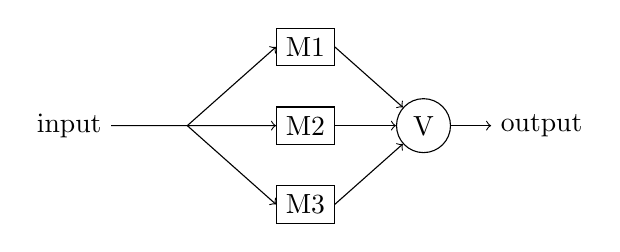
\begin{tikzpicture}
\node[draw,rectangle] (M1) at (0,1) {M1};
\node[draw,rectangle] (M2) at (0,0) {M2};
\node[draw,rectangle] (M3) at (0,-1) {M3};
\node[draw,circle] (V) at (1.5,0) {V};
\node (O) at (3,0) {output};
\node (I) at (-3,0) {input};
\coordinate (J) at (-1.5,0);
\draw[->] (I.east) -- (J) -- (M1.west);
\draw[<->] (M2.west) -- (J) -- (M3.west);
\draw[->] (M1.east) -- (V);
\draw[->] (M2.east) -- (V);
\draw[->] (M3.east) -- (V);
\draw[->] (V) -- (O.west);
\end{tikzpicture}